\begin{figure}
    \centering
    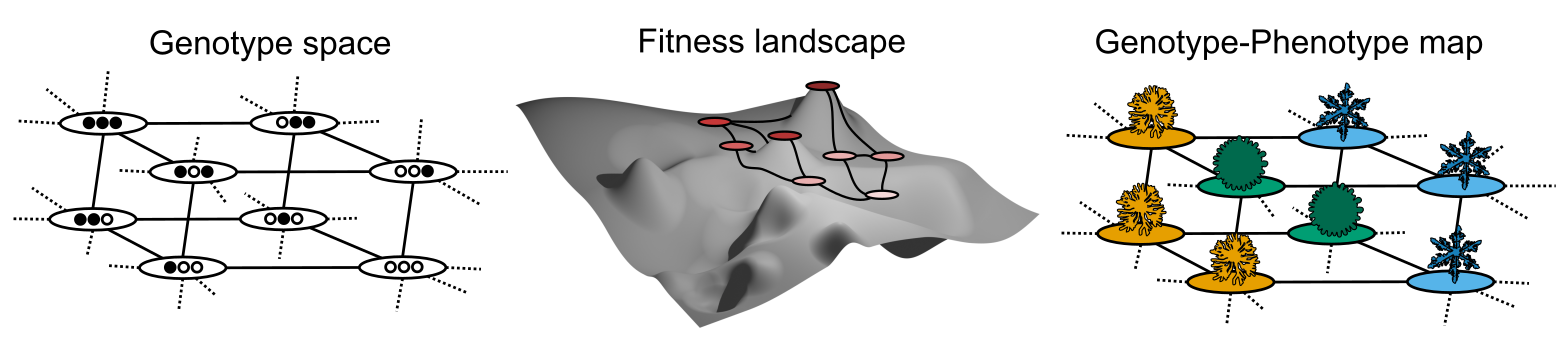
\includegraphics[width=1.0\linewidth]{img/fitness_landscapes.png}
    \caption{%
\textbf{Adaptive Landscapes}.
The \textit{genotype space} (left) is a network of genotypes, with edges connecting genotypes that differ by a single mutation.
A \textit{fitness landscape} (middle) is induced on this space when each genotype is assigned a value denoting its reproductive success in an environment.
Alternatively, the genotypes may be assigned ``phenotypes'' that denote expressed traits, producing a \textit{genotype-phenotype map} (right)
}
\label{fig:fitness_landscapes}
\end{figure}
